\documentclass[a4paper, amsfonts, amssymb, amsmath, reprint, showkeys, nofootinbib, twoside]{revtex4-1}
\usepackage[english]{babel}
\usepackage[utf8]{inputenc}
\usepackage[colorinlistoftodos, color=green!40, prependcaption]{todonotes}
\usepackage[pdftex, pdftitle={Article}, pdfauthor={Author}]{hyperref}
\usepackage{amsthm}
\usepackage{mathtools}
\usepackage{physics}
\usepackage{xcolor}
\usepackage{caption}
\usepackage{hyperref}
%\hypersetup{colorlinks=true, linkcolor=blue, urlcolor = blue}
\usepackage{amsmath}
\usepackage{amssymb}
\usepackage{graphicx}
\graphicspath{Images}
\usepackage[left=23mm,right=13mm,top=35mm,columnsep=15pt]{geometry} 
\usepackage{adjustbox}
\usepackage{placeins}
\usepackage[T1]{fontenc}
\usepackage{float}
%\usepackage{longtable}
\usepackage{csquotes}
\usepackage{refstyle}
\usepackage{lipsum}

\begin{document}

\title{Study of Lock-In Amplifier}
\author{Swaroop Ramakant Avarsekar}
\email{swaroop.avarsekar@niser.ac.in}
\affiliation{School of Physical Sciences, National Institute of Science Education and Research, HBNI, Jatni -752050, India}
\date{\today}

	
\begin{abstract}
The lock-in amplifier measures small voltages as it selectively amplifies the required signal from noise. It uses principle of phase sensitive detection. It can be used in many ways. In this experiment we use this to find the amplification factor and determine the mutual inductance of a coil and determine the low resistance.  We obtained the amplification factor as (1.61$\pm$ 0.06) $\times$ $10^3$ , mutual inductance of given coil as $(123.98\pm4.67)$ $\mu H$ and low resistance as $0.38\pm0.03$ $\Omega$.
\end{abstract}
	
\keywords{Lock-In amplifier, Mutual inductance, Lissajous figure}
	
\maketitle

\section{Introduction and Theory}
Amplifiers are used to amplify the weak AC signal with the amplification factor. However amplifier also amplifies noise. Amplifiers have a bandwidth of several kilohertz. Usually noise is present over a
range of frequencies while the signal is at a single frequency. If the signal is very weak,
amplification alone will not enable us to pick out the signal against noise. To reduce the noise we either reduce the temperature T or reduce the bandwidth W of the amplifier. For detecting very weak signals at room temperature we have to effectively reduce the bandwidth to a few Hertz though the amplifier has a large bandwidth in kilohertz range. This is achieved by Phase Sensitive Detection (PSD). A lock-in amplifier (LIA) uses principle of PSD where reference signal of same frequency is provided as that of main signal producing maximum DC output when reference signal is in phase with the main signal.

\begin{figure}[h]
	\centering
	\includegraphics[width=8cm]{f2} 
	\caption{Block diagram of Lock In Amplifier}
	\label{f2}
\end{figure}

LIA filters out noise in the input using PSD with AD 630 chip, which consists of  two identical amplifiers. 
One is a direct amplifier. This means that the
output is in phase with the input. The other is an inverse amplifier i.e. the output is $180^{\circ}$
out of phase with the input. There is a switch operated by a comparator. The comparator senses the reference signal. When the reference signal is positive (i.e. for time t, 0<t<T/2) the comparator connects the weak signal $V_signal$ to the direct amplifier so that the output of the amplifier is 

\begin{equation}
	V_{out}=\mu V_{signal}
\end{equation}

When the reference signal is negative for time between T/2 to T, the weak signal is connected to inverse amplifier so that output is 
\begin{equation}
	V_{out}=-\mu V_{signal}
\end{equation}
where $\mu$ is the amplification factor of LIA

If we introduce a circuit to phase shift the reference signal and then send the phase shifted
reference signal to the comparator in AD 630, the output DC voltage will vary as the phase shift is increased from zero. It will reach a maximum when the reference signal is phase shifted by $\phi$ and the phase-shifted reference signal is in phase with the weak signal
$V_{signal}$. Then the output voltage will look like the one shown in Figure (\ref{f1}). The
average DC voltage, $V_{DC}$, will then reach a maximum value $2.\mu.V_{out}/\pi$.
It is called phase sensitive detection and the amplifier a lock-in amplifier because we make the weak signal lock in phase with the phase-shifted reference to give
maximum DC output voltage. If we measure on an oscilloscope how much we have to shift the phase of the reference signal to get maximum DC output, that gives the phase difference between effect and cause.

\begin{figure}[h]
		\centering
		\includegraphics[width=8cm]{f1} 
		\caption{Amplified output signal when reference signal is phase shifted by $\phi$ and fed to AD 630 chip }
		\label{f1}
\end{figure}

To calibrate the LIA, we calculate the amplification factor $\mu$ of the instrument by measuring output DC voltage of LIA for known AC signal as function of frequency.

\begin{equation}
	 \text{Amplification factor}, \mu=V_{DC}/V_{AC}
\end{equation}

When two coils are placed beside each other with AC voltage passing through primary coil, we induce emf in secondary coil with same frequency f. If the primary current varies as 
\begin{equation}
	I=I_o.sin(2\pi f t)
\end{equation}
Emf induced in secondary coil is 
\begin{equation}
	V=-M\frac{dI}{dt}=-2\pi M f I_o sin(2 \pi f t+\pi/2 )
\end{equation}

Therefore, the the phase difference between the primary current and the induced emf is $\pi/2$, the secondary emf is proportional to the amplitude $I_o$ of the primary current and the induced emf is proportional to the frequency f. 

The phase shift knob of the lock in amplifier can be used
to correct the phase difference. Then, the mutual inductance of the coil is give by
\begin{equation}
	M=R.\beta  /2 \pi \mu
\end{equation}

where M is the mutual inductance of the coil, $\mu$ is 
amplification factor of the LIA, R is the resistance in the primary circuit and $\beta$ is the slope of plot between slope of $V_{DC}$ and $V_{AC}$ versus frequency.

\begin{figure}[H]
	\centering
	\includegraphics[width=8cm]{f3} 
	\caption{Circuit diagram for measuring low resistance by LIA}
	\label{f3}
\end{figure}

The lock in amplifier can also be used to measure a low resistance by connecting the amplifier with a resistance box. As show in in figure (\ref{f3}) Here, the voltage across the 100$\Omega$ resistor serves as
the reference signal and the 4.7 kΩ resistor limits the current through the wire to a few hundred micro amperes when the signal generator output is connected to the terminals of the box. The value of low resistance can be then calculated by-

\begin{equation}
	\frac{d V_{DC}}{dV_{AC}}=\frac{\mu r}{R}
\end{equation}

where r is the low resistance and R is the total resistance of primary circuit.

\section{Experiment}
\begin{figure}[h]
	\centering
	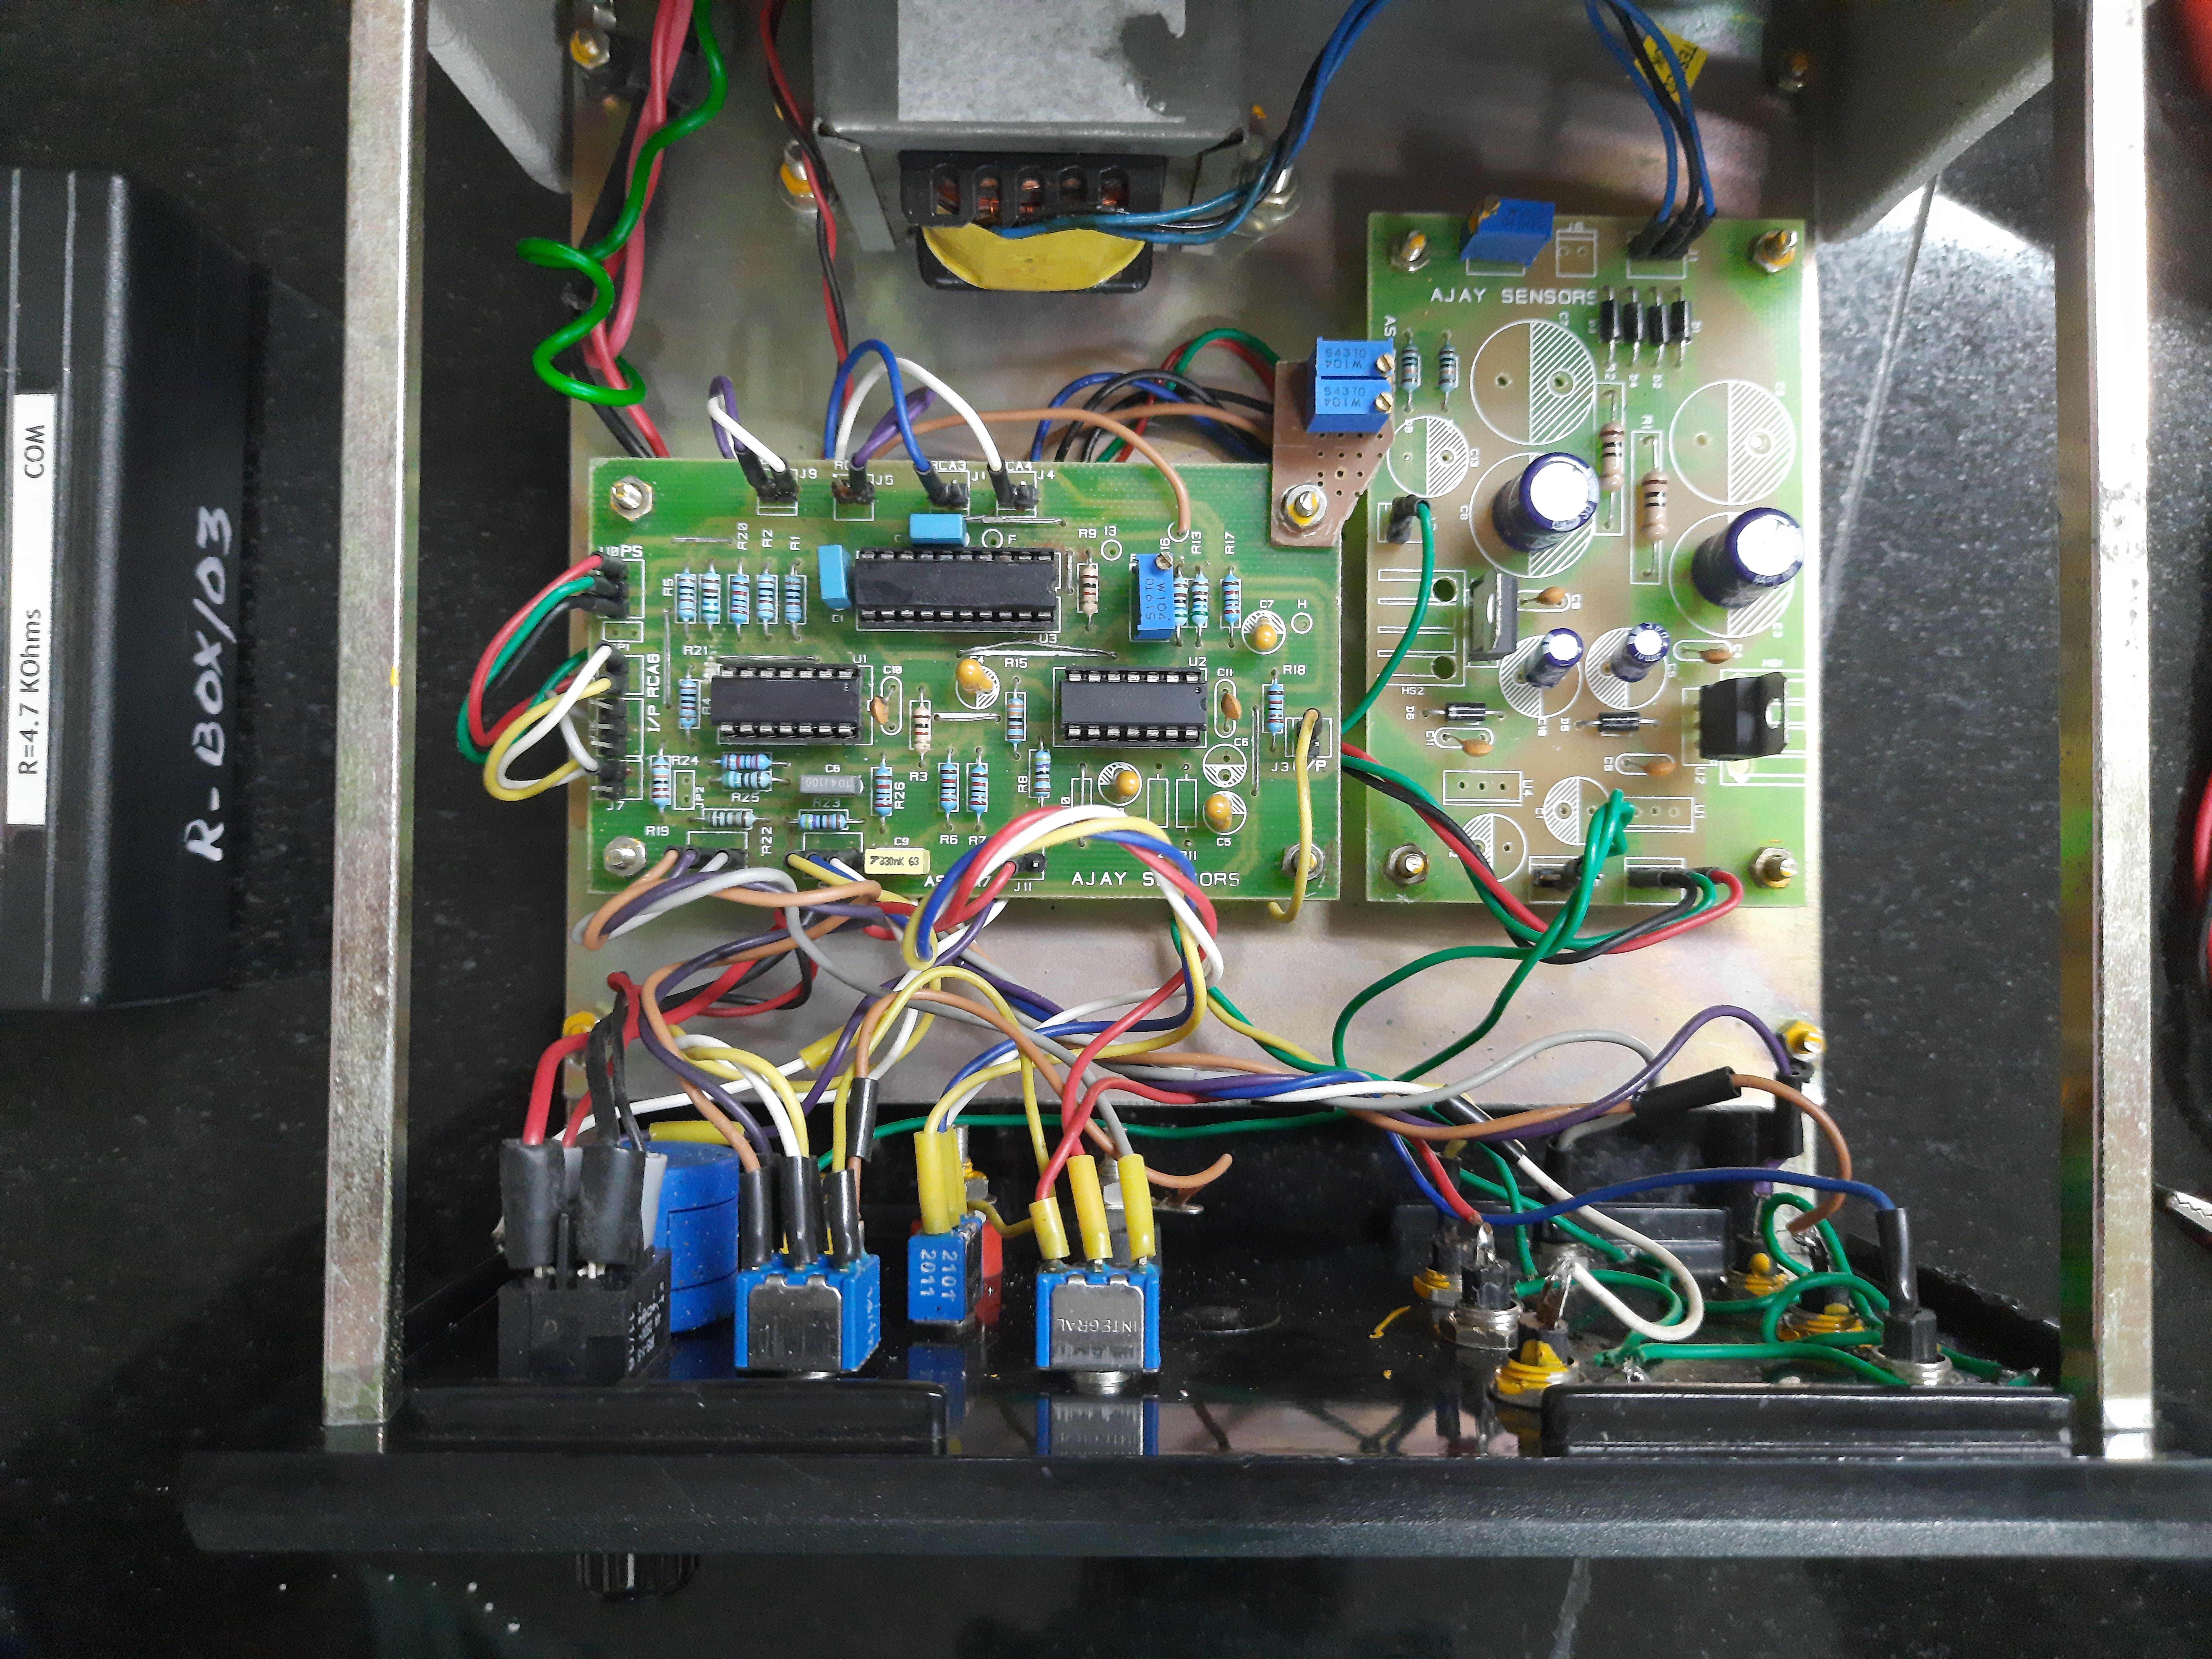
\includegraphics[width=8cm]{f4} 
	\caption{Circuit in LIA}
	\label{f4}
\end{figure}
\subsection{Apparatus}
The apparatus required for these experiments are Lock In amplifier, signal generator, digital Multi-meter, two channel digital Oscilloscope, Mutual inductance coil, low resistance box, crocodile clips and connecting wires
\subsection{Procedure}
\subsubsection{Calibration of LIA}
 A signal generator is connected to the RCA socket marked SIG GEN at the bottom of the front panel of the LIA. The internal circuit is connected after turning the SW1 and SW2 switches to calibration CAL. The frequency in the signal generator is set to 500Hz with an amplitude of 4V, $V_{app}$. Inside the Lock in amplifier, this voltage will be applied to three resistances in
 series, namely 220 k $\Omega$, 10 $\Omega$ and 5 k $\Omega$. The voltage across 10 Ohms will be  $V_{signal}$ is
 \begin{equation}
 	V_{signal}=V_{app}.10/(225\times10^3)=44.4 V_{app} \mu V
 \end{equation}
 
 The SW3 switch is turned up and the phase shift knob is turned to zero. The RCA sockets marked REF and REF‘ is connected to the two channels of the oscilloscope. Turn the phase adjustment potentiometer knob to the right extreme and wait till the DMM connected to the output socket of the lock in shows a steady DC value. At the right extreme the phase difference between the signal and the reference is zero. Note the reading on the DMM. This is called $V_{DC}$. Repeat the above steps with different voltage from 1.5 V to 4 V with the same frequency. Repeat the entire procedure for different frequencies and
plot the graph between $V_{DC}$ and $V_{signal}$ find their slope to obtain the amplification factor. 

\subsubsection{Measuring Mutual Inductance of coil}
Connect the inductance coil with LIA as mentioned in the setup section of this report with SW1 and SW2 switches towards EXT. Connect the two RCA sockets marked REF and REF’ on the front panel of the LIA to the two channels of an oscilloscope. Connect the signal generator to the primary coil and switch
on the signal generator. Set the amplitude of the signal to 4 V and frequency to 400Hz. Adjust the phase shift knob such that, the reading on the
DMM reaches maximum and the phase difference in
the oscilloscope reaches 900. Vary the amplitude from the signal generator between
1.5V and 4V. Repeat the entire procedure for different frequencies and plot the graph between $V_{DC}$ and $V_{AC}$, find their slope and mutual inductance.

\subsubsection{Measuring low resistance}
Connect the resistance box with LIA as mentioned in the
setup section of this report with SW1 and SW2 switches
towards EXT. Switch on the signal generator with a frequency of 200Hz and amplitude of 4.5 V. Turn the phase adjusting knob to the extreme right and
measure the value of both DC output voltage and the AC
voltage given with the input varying from 2 V to 4.5 V. Repeat the entire procedure for different frequencies and
plot the graph between $V_{DC}$ and $V_{AC}$ to find their slope, using which, calculate the value of the low resistance.

\begin{figure}[h]
	\centering
	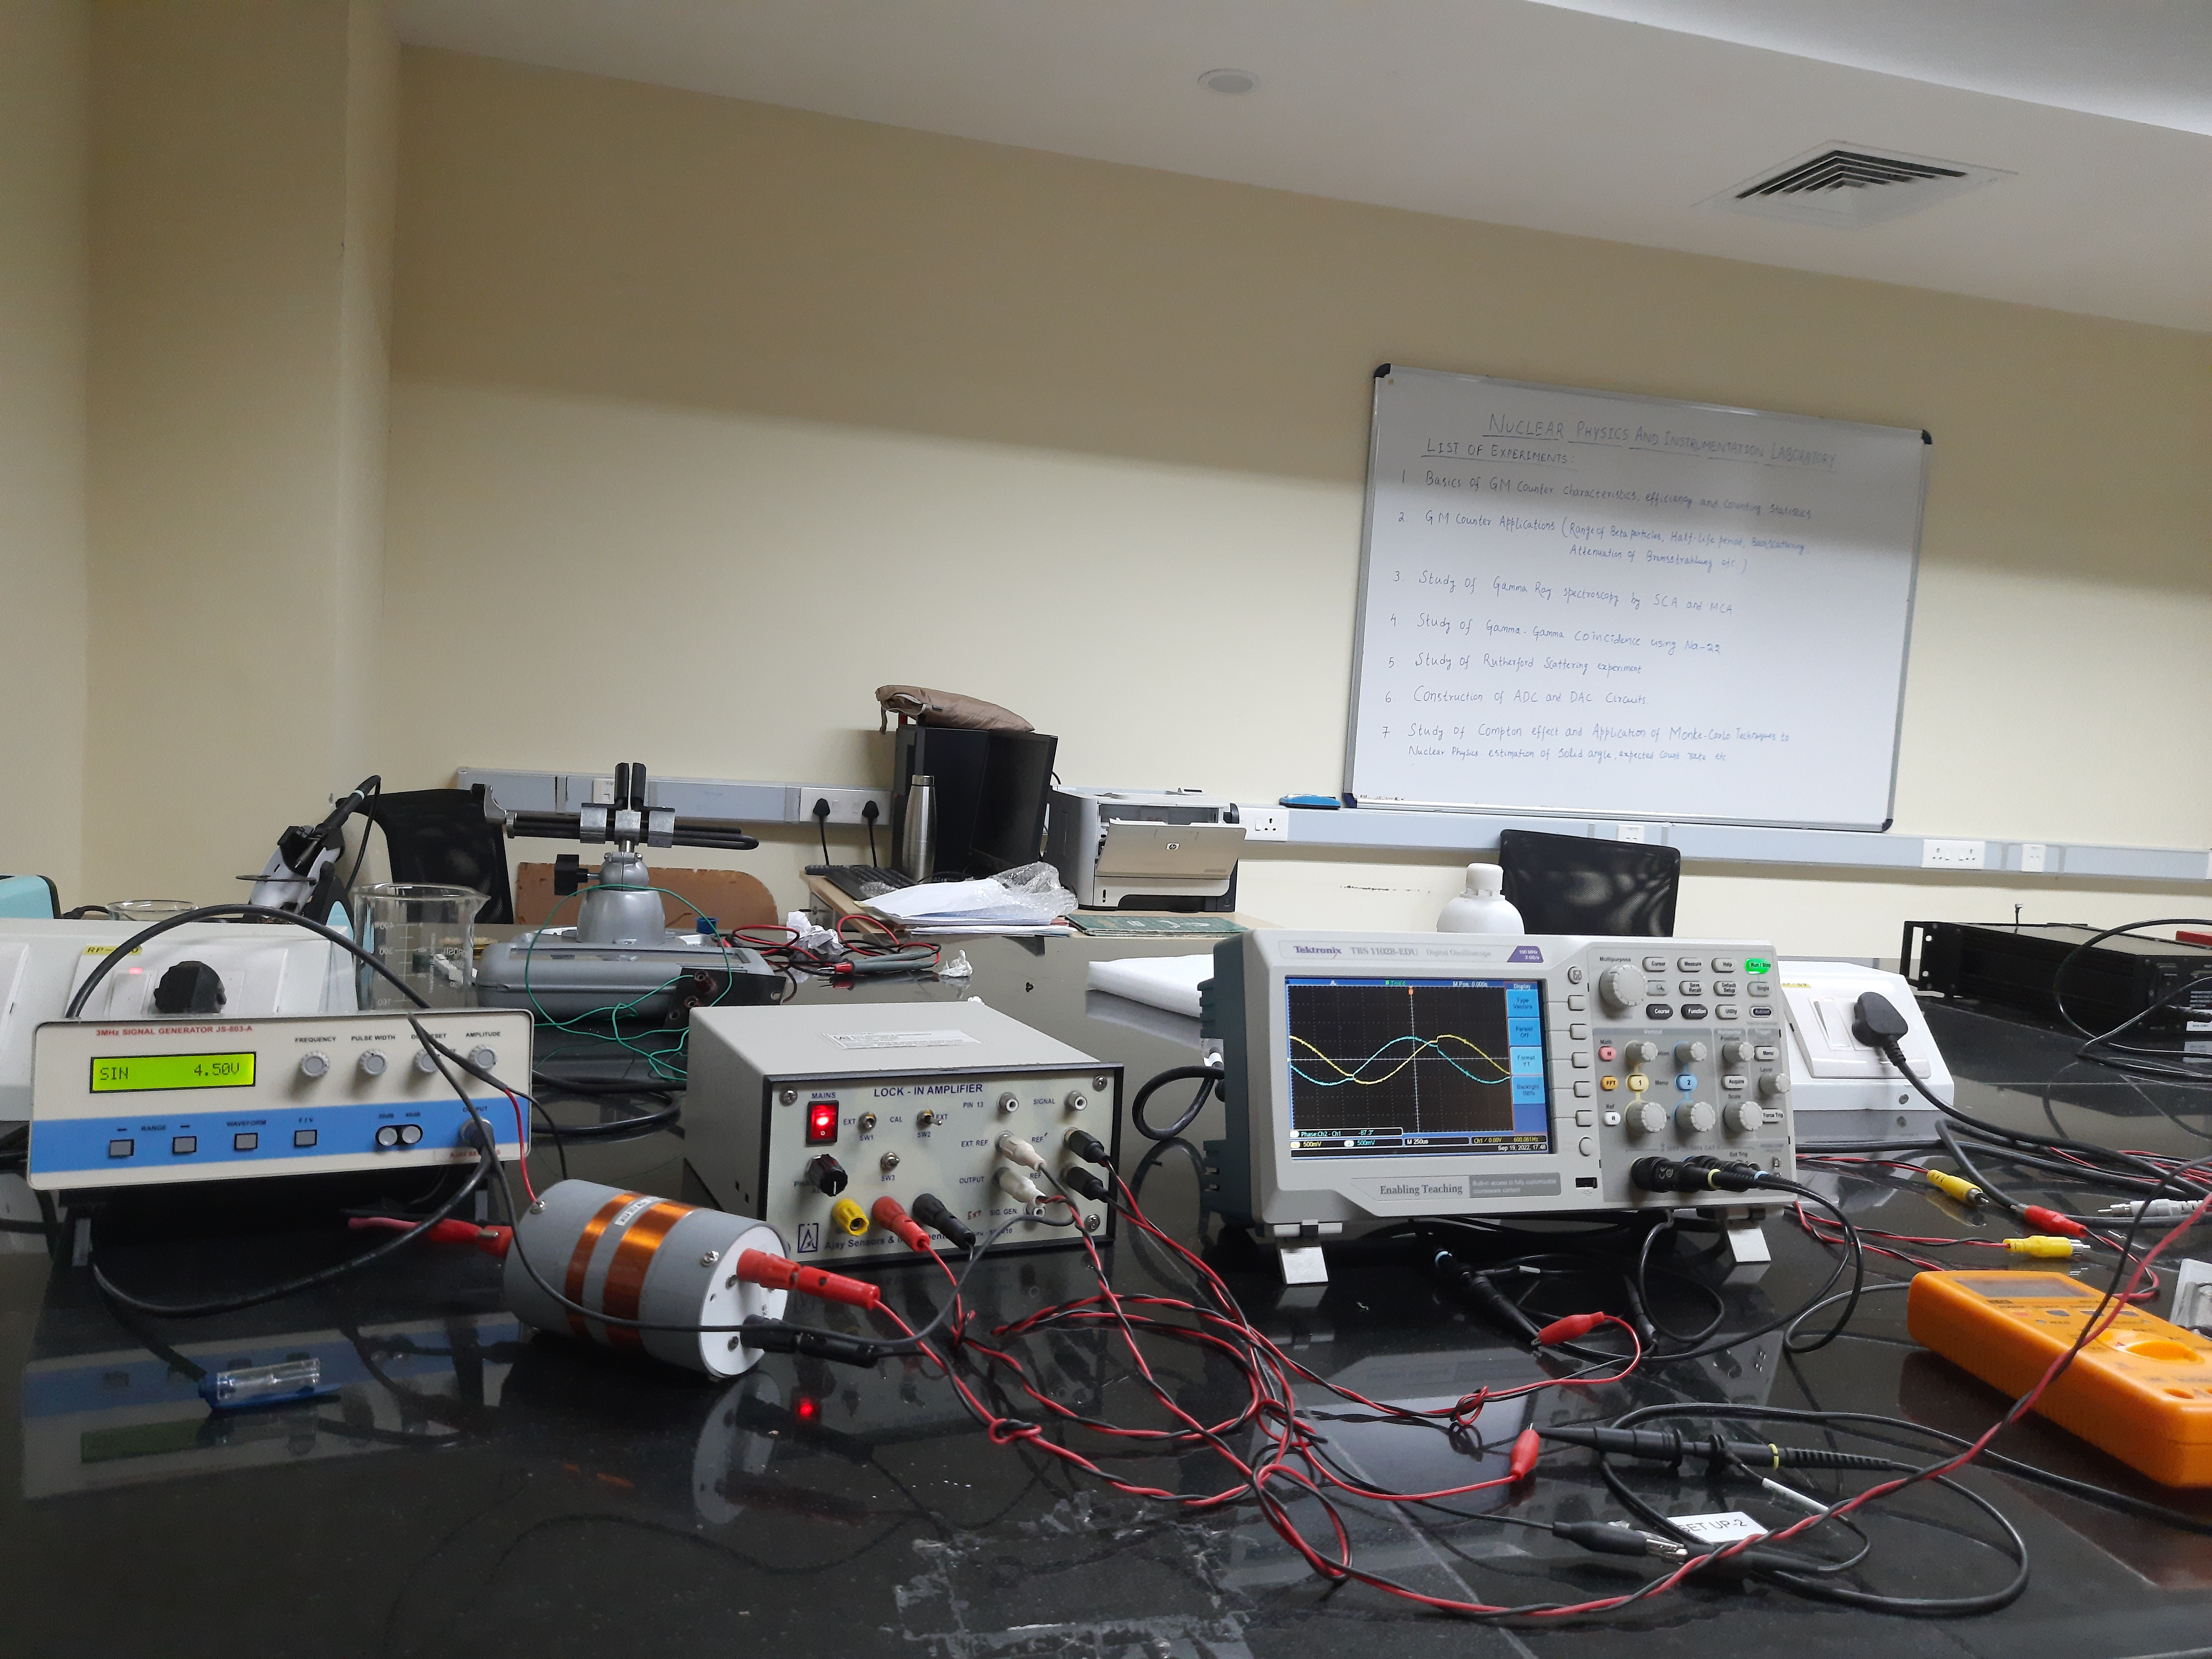
\includegraphics[width=8cm]{f5} 
	\caption{Experimental setup to determine mutual inductance of the coil.}
	\label{f5}
\end{figure}

\section{Observation and Analysis}

\begin{figure}[H]
	\centering
	\includegraphics[width=8cm]{f6} 
	\caption{Plot of $V_{signal}$ versus $V_{DC}$ for calculating amplification factor}
	\label{f6}
\end{figure}

To calculate the amplification factor for LIA, we plot the graph for $V_{signal}$ versus $V_{DC}$. The slope of this plot gives the value of amplification factor ($\mu$). Since, the $\mu$ is frequency independent, we can take the average of all the $\mu$ obtained for different frequencies. Giving the net amplification factor $\mu$ =(1.61$\pm$ 0.06) $\times$ $10^3$

\begin{figure}[h]
	\centering
	\includegraphics[width=8cm]{f7} 
	\caption{Plot of $V_{AC}$ versus $V_{DC}$ for calculating mutual inductance of coil.}
	\label{f7}
\end{figure}

\begin{figure}[h]
	\centering
	\includegraphics[width=8cm]{f8} 
	\caption{Plot of frequency versus slope}
	\label{f8}
\end{figure}

To calculate the mutual inductance, we plot $V_{AC}$ versus $V_{DC}$ for different frequencies and record the slope. Again we plot these slope versus frequency to calculate the $\beta$. From the plot of frequency versus slope, we get $\beta$ as (2.613$\pm$0.018)$\times$ $10^{-4}$. 

\begin{equation}
	M=R.\beta  /2 \pi \mu
\end{equation}

\begin{equation}
	M=4.8\times10^3\times2.613\times 10^{-4}/(2 \pi. 1.61\times10^3)
\end{equation}

Error in M,
\begin{equation}
\frac{\delta M}{M}= \sqrt{\left(\frac{\delta \beta}{\beta}\right)^2+\left(\frac{\delta \mu}{\mu}\right)^2}
\end{equation}

From above calculation, we get M=$(123.98\pm4.67)$ $\mu H$.

\begin{figure}[H]
	\centering
	\includegraphics[width=8cm]{f9} 
	\caption{Plot of $V_{AC}$ versus $V_{DC} for calculating low resistance$}
	\label{f9}
\end{figure}

The graph of $V_{AC}$ versus $V_{DC}$ is plotted for different frequencies. Then the slope is averaged out since it is independent of frequency. Slope=$0.1273\pm0.0082$

\begin{equation}
	\text{slope}=\mu r/R
\end{equation}

Where R=4.8 k $\Omega$ 

Error in r,
\begin{equation}
	\frac{\delta r}{r}= \sqrt{\left(\frac{\delta slope}{slope}\right)^2+\left(\frac{\delta \mu}{\mu}\right)^2}
\end{equation}

Therefore, r=$0.38\pm0.03$ $\Omega$
\section{Conclusion}
The amplification factor of LIA was found to be (1.61$\pm$ 0.06) $\times$ $10^3$ for the different frequencies by calibrating LIA. The LIA was used to find the mutual inductance of a coil which turned out to be  M=$(123.98\pm4.67)$ $\mu H$. We also observed that the emf is $\pi$/2 out of phase with the current in the primary coil, emf is proportional to current in primary coil and frequency. We also determined the low resistance,r, less than 1 $\Omega$ from LIA. We obtained r as $0.38\pm0.03$ $\Omega$. 
The experiment gave us the acceptable values as compared to given values for the coils and resistance. Few errors may have propped up due to human errors while measuring the voltages across DMM, unstable values in DMM resulted in approximating the values. Instrumental errors and loose connections also played role for adding the error to the experiment. The errors can be minimized by increasing the number of readings for each frequencies. 

\section{References}
\begin{enumerate}
\item{\url{https://www.niser.ac.in/sps/sites/default/files/basic_page/Lockinamplifier_manual.pdf}}

\end{enumerate}

\end{document}